\chapter{Experiments and Evaluation} \label{the-chapter-5}

In this chapter, we discuss the experiments conducted by us to evaluate the tagging performance of HeidelTime using our improved automatically developed resources and the results obtained.
 
\section{Evaluation Approach}
To evaluate our improved automatically developed resources, we use different versions of our created resources. For instance, we use the new resources that only have inflections, the new resources that have both inflections and learned frequently occurring pattern rules in them. Furthermore, we run evaluations on temporally annotated corpora and do analysis on Wikipedia dumps. As explained in Subsection \ref{the-chapter-3-alltc}, only a few languages have temporally annotated corpora, so we will do analysis on Wikipedia dumps for few languages that lack such corpora.

\textbf{Resources Versions}\\
In the following table, we summarize the different versions of HeidelTime resources that we will be evaluating. 

\begin{table}[H]
	\centering
	\rowcolors{1}{}{cream}
	\begin{threeparttable}
		\begin{tabularx}{\linewidth}{||>{\raggedright\arraybackslash}p{.7in} | >{\raggedright\arraybackslash}X |  >{\raggedright\arraybackslash}p{1.2in}||} 
			\hline
			\textbf{Version} & \textbf{About} & \textbf{Reference} \\ [0.5ex] 
			\hline\hline
			2.2.1 & the automatically developed resources with the version 2.2.1 release of HeidelTime (this version disregards inflections)  & Str\"otgen and Gertz in \cite{DBLP:conf/emnlp/StrotgenG15}, and Section \ref{multilingual-ht-model} \\ 
			\hline
			2.x & this version uses wiktionary to get inflections -- and the rules of unsegmented languages do not use space as separator between rePatterns & Subsection \ref{sec4b1} and Section \ref{sec4c} \\ 
			\hline
			2.x-wv & this version uses word vectors to get inflections - (word vectors)& Subsection \ref{sec4b2} \\ 
			\hline
			2.x-afr & same as version 2.x with the addition, i.e., this version has frequently occurring patterns learned as rules - (appended frequent rules) & Section \ref{sec4d} \\ 
			\hline
		\end{tabularx}
%		\begin{tablenotes}
%			\item[1] for unsegmented languages, the rules do not use space as separator between rePatterns
%		\end{tablenotes}
	\end{threeparttable}
	\caption{Summary of different HeidelTime versions for automatically developed resources.}
	\label{table:5a}
\end{table}

\section{Evaluating Using Temporal Corpora}
To evaluate the tagging performance of HeidelTime using the automatically developed resources, we use the following measures, i.e., precision, recall and f1-score. These measures can be better understood with the help of a confusion matrix that describe the decisions of a temporal tagger against the ground truth \cite{DBLP:series/synthesis/2016Strotgen}.

\begin{table}[H]
	\centering
	\begin{threeparttable}
	\begin{tabularx}{380pt}{>{\raggedright\arraybackslash}X|>{\raggedright\arraybackslash}X  >{\raggedright\arraybackslash}X }
		
		\multirow{2}{*}{} & \multicolumn{2}{l}{\textbf{Gold Standard (Ground Truth)}} \\
		\textbf{System Prediction}	 & Positive & Negative  \\ 
		\hline
		Positive & TP & FP \\ 
		Negative & FN & TN \\ 
		
	\end{tabularx}
%		\begin{tablenotes}
%			\item[1] for unsegmented languages, the rules do not use space as separator between rePatterns
%		\end{tablenotes}
	\end{threeparttable}
	\caption{Confusion matrix for temporal tagger decisions.}
	\label{table:5b}
\end{table}

The Table \ref{table:5b}, summarizes the four classes that each of the decision of a temporal tagger can be fall in. 
\begin{itemize}
	\item True Positive (TP): identified as a positive by the system, and was also positive in the gold standard (correct decision)
	\item False Positive (FP): identified as a positive by the system, but was negative in the gold standard (incorrect decision)
	\item False Negative (FN): identified as a negative by the system, but was positive in the gold standard (incorrect decision)
	\item True Negative (TN): identified as a negative by the system, and was also negative in gold standard (correct decision)
\end{itemize}

\subsection{Evaluation Measures}
The three frequently used measures for evaluating performance of temporal taggers on temporally annotated corpara are: precision, recall and f1-score. 

\textbf{Precision}\\
For the task of temporal expression extraction, precision would be the fraction of correctly extracted temporal expressions out of all extracted temporal expressions. And for the task of temporal expression normalization, precision would be the fraction of correctly normalized temporal expressions out of all normalized temporal expressions. It is calcuated using the following formula:
$$P = \frac{TP}{TP+FP}$$
It is evident that a system can achieve higher precision by extracting a few temporal expressions only. For instance, if corpora has 100 true temporal expressions, and system extracts 10 expressions and 9 of them are indeed temporal expressions, the precision of system will be $\frac{9}{10} = 0.9$. As we can see from this example, that a system can achieve high precision even if it extract a small part of all temporal expressions in a corpora (only 9 out of 100 in this example). So it is not good to only rely on precision to evaluate a system. 

\textbf{Recall}\\
For the task of temporal expression extraction, recall would be the fraction of correctly extracted temporal expressions out of all true temporal expressions. And for the task of temporal expression normalization, recall would be the fraction of correctly normalized temporal expressions out of all true normalized temporal expressions. It is calculated using the following formula:
$$R = \frac{TP}{TP+FN}$$
It is evident that a system can achieve higher recall by extracting all expressions in corpora as temporal expressions. Recall is a non-decreasing function of the number of expressions extracted or normalized. So it is not good to only rely on recall to evaluate a system. 

%\begin{table}[H]
%	\centering
%	\rowcolors{1}{}{cream}
%	\begin{threeparttable}
%		\begin{tabularx}{\linewidth}{||>{\raggedright\arraybackslash}p{1.6in} | >{\raggedright\arraybackslash}X |  >{\raggedright\arraybackslash}X||} 
%			\hline
%			\textbf{-} & \textbf{Is Temporal Expression} & \textbf{Is Not Temporal Expression} \\ [0.5ex] 
%			\hline\hline
%			Extracted & tp  & fp \\ 
%			\hline
%			Not Extracted & fn & tn \\ 
%			\hline
%		\end{tabularx}
%		%		\begin{tablenotes}
%		%			\item[1] for unsegmented languages, the rules do not use space as separator between rePatterns
%		%		\end{tablenotes}
%	\end{threeparttable}
%	\caption{Decisions of a temporal tagger - confusion matrix.}
%	\label{table:5b}
%\end{table}

\textbf{F\textsubscript{1} score}\\
F\textsubscript{1} score combines both precision and recall to balance out their shortcomings. It is given by the following formula: 
$$F_1 = \frac{2\times P\times R}{P+R}$$ 
This measure can be seen as a harmonic mean of precision and recall. F\textsubscript{1} score can be seen as a balancing measure which balances out the skew in our system results if we rely on only precision or only recall.

\subsection{Strict and Relaxed Matching}
As temporal expressions may consist of more than one consecutive tokens, so there is a possibility that an extracted temporal expression might overlap with another extracted temporal expression \cite{DBLP:series/synthesis/2016Strotgen}. Moreover, such temporal expressions might be extracted completely or some part of them might be extracted. Due to this temporal taggers can be evaluated using either strict matching or relaxed matching. We demonstrate this with the following example:

\begin{mdframed}[style=MyFrame]
	\raggedright{
		\textbf{Gold Standard}\\
		The car that was lost on <TIMEX3>\underline{1st June}</TIMEX3> was found <TIMEX3>\underline{about three weeks later}</TIMEX3>. 
		
		\textbf{Annotated by a tagger}\\
		The car that was lost on <TIMEX3>\underline{1st June}</TIMEX3> was found about <TIMEX3>\underline{three weeks later}</TIMEX3>. 
	}
\end{mdframed}

In above example, we can see that the gold standard has two temporal expressions, i.e.,  ``1st June" and ``about three weeks later", and a tagger tags the first temporal expression completely and the second one partially. If we evaluate the tagger's extraction performance using strict matching, there is 1 true positive (``1st June"), 1 false positive (``three weeks later") and 1 false negative (``about three weeks later"). However, using relaxed matching there are 2 true positives (``1st June" and ``three weeks later"). It is to be noted that in relaxed matching the second temporal expressions that was annotated by the tagger, was considered a true positive because it overlapped with its annotation in the gold standard. For a detailed discussion about strict and relaxed matching and issues in evaluating temporal taggers, we refer the reader to the book \cite{DBLP:series/synthesis/2016Strotgen}.

The organizers of TempEval-3, consider \textit{value f1-score with relaxed matching} as the most informative measure to evaluate temporal taggers. That is, for extraction consider relaxed matching, and for normalization consider correct value normalization. 

\subsection{Results and Discussion}
The temporal corpora we will be evaluating on are summarized in the Subsection \ref{tactac}. Following, we disucss the evaluation results. 

\textbf{The AncientTimes Corpus - Several Languages}\\
In the following table, we summarize the evaluation results for AncientTimes corpus. 

\begin{table}[H]
	\centering
%	\rowcolors{1}{}{cream}
	\begin{threeparttable}
		\begin{tabularx}{\linewidth}{|| >{\raggedright\arraybackslash}p{.5in} >{\raggedright\arraybackslash}p{.5in} | X X X | X X X | X X ||} 
			\hline
			\multicolumn{2}{||c}{\multirow{2}{*}{}} & \multicolumn{3}{c}{Strict Extraction} & \multicolumn{3}{c}{Relaxed Extraction} & \multicolumn{2}{c||}{Attribute} \\ [0.5ex] 
%			\hline
			\textbf{corpus} & \textbf{version} & \textbf{P} & \textbf{R} & \textbf{F1} & \textbf{P} & \textbf{R} & \textbf{F1} & \textbf{value F1} & \textbf{type F1}\\ 
			\hline\hline
			
			\multirow{3}{\linewidth}{\scriptsize{Ancient Times German}} & 2.2.1 & 76.64 & 45.05 & 56.75 & 100.0 & 58.79 & 74.05 & 67.82 & 73.36 \\ 
			\cline{2-10} & 2.x & 75.0 & 47.8 & 58.39 & 100.0 & 63.74 & 77.85 & 67.79 & 73.15 \\
			\cline{2-10} & 2.x-wv & 61.9 & 7.14 & 12.81 & 100.0 & 11.54 & 20.69 & 11.82 & 20.69 \\  
			\cline{2-10} & 2.x-afr & 74.36 & 47.8 & 58.19 & 100.0 & 64.29 & \textbf{78.26} & \textbf{68.23} & 73.58 \\ 
			\hline\hline
			
			\multirow{3}{\linewidth}{\scriptsize{Ancient Times Spanish}} & 2.2.1 & 23.61 & 8.06 & 12.01 & 58.33 & 19.91 & 29.68 & 16.25 & 28.98 \\ 
			\cline{2-10} & 2.x & 23.61 & 8.06 & 12.01 & 58.33 & 19.91 & 29.68 & \textbf{16.25} & 28.98 \\ 
			\cline{2-10} & 2.x-wv & 27.45 & 6.64 & 10.69 & 50.98 & 12.32 & 19.85 & 16.03 & 19.85 \\  
			\cline{2-10} & 2.x-afr & 22.67 & 8.06 & 11.89 & 60.0 & 21.33 & \textbf{31.47} & 16.08 & 30.77 \\ 
			\hline\hline
			
			\multirow{3}{\linewidth}{\scriptsize{Ancient Times French}} & 2.2.1 & 59.52 & 26.32 & 36.5 & 99.21 & 43.86 & 60.83 & 53.53 & 60.83 \\ 
			\cline{2-10} & 2.x & 59.52 & 26.32 & 36.5 & 99.21 & 43.86 & \textbf{60.83} & \textbf{53.53} & 60.83 \\
			\cline{2-10} & 2.x-wv & 70.45 & 10.88 & 18.84 & 100.0 & 15.44 & 26.75 & 20.67 & 24.92 \\
			\cline{2-10} & 2.x-afr & 59.52 & 26.32 & 36.5 & 99.21 & 43.86 & 60.83 & 50.61 & 58.39 \\
			\hline\hline
			
			\multirow{3}{\linewidth}{\scriptsize{Ancient Times Dutch}} & 2.2.1 & 62.79 & 21.6 & 32.14 & 90.7 & 31.2 & 46.43 & 22.62 & 42.86 \\ 
			\cline{2-10} & 2.x & 62.79 & 21.6 & 32.14 & 90.7 & 31.2 & 46.43 & 22.62 & 42.86 \\
			\cline{2-10} & 2.x-wv & 53.85 & 11.2 & 18.54 & 84.62 & 17.6 & 29.14 & 22.52 & 27.81 \\
			\cline{2-10} & 2.x-afr & 62.79 & 21.6 & 32.14 & 90.7 & 31.2 & \textbf{46.43} & \textbf{22.62} & 42.86 \\ 
			\hline\hline
			
			\multirow{3}{\linewidth}{\scriptsize{Ancient Times Italian}} & 2.2.1 & 68.99 & 38.86 & 49.72 & 96.9 & 54.59 & 69.83 & 57.54 & 69.27 \\ 
			\cline{2-10} & 2.x & 68.99 & 38.86 & 49.72 & 96.9 & 54.59 & 69.83 & 57.54 & 69.27 \\
			\cline{2-10} & 2.x-wv & 67.39 & 13.54 & 22.55 & 95.65 & 19.21 & 32.0 & 20.36 & 31.27 \\
			\cline{2-10} & 2.x-afr & 64.49 & 38.86 & 48.5 & 97.1 & 58.52 & \textbf{73.02} & \textbf{58.86} & 71.93 \\ 
			\hline\hline
			
			\multirow{3}{\linewidth}{\scriptsize{Ancient Times Vietnamese}} & 2.2.1 & 2.38 & 0.86 & 1.27 & 69.05 & 25.0 & 36.71 & 5.06 & 18.99 \\ 
			\cline{2-10} & 2.x & 2.38 & 0.86 & 1.27 & 69.05 & 25.0 & \textbf{36.71} & 1.27 & 18.99 \\ 
			\cline{2-10} & 2.x-wv & 2.94 & 0.86 & 1.33 & 76.47 & 22.41 & 34.67 & \textbf{6.67} & 6.67 \\
			\cline{2-10} & 2.x-afr & 2.33 & 0.86 & 1.26 & 67.44 & 25.0 & 36.48 & 6.29 & 16.35 \\ 
			\hline\hline
			
			\multirow{3}{\linewidth}{\scriptsize{Ancient Times Arabic}} & 2.2.1 & 12.5 & 0.99 & 1.83 & 62.5 & 4.95 & \textbf{9.17} & \textbf{3.67} & 7.34 \\ 
			\cline{2-10} & 2.x &  0.0 & 0.0 & 0.0 & 50.0 & 1.98 & 3.81 & 1.9 & 3.81 \\ 
			\cline{2-10} & 2.x-wv & 0.0 & 0.0 & 0.0 & 16.67 & 1.98 & 3.54 & 0.0 & 3.54 \\
			\cline{2-10} & 2.x-afr &  0.0 & 0.0 & 0.0 & 50.0 & 1.98 & 3.81 & 1.9 & 3.81 \\  
			\hline
				
		\end{tabularx}
		%		\begin{tablenotes}
		%			\item[1] for unsegmented languages, the rules do not use space as separator between rePatterns
		%		\end{tablenotes}
	\end{threeparttable}
	\caption{Evaluation results for AncientTimes corpora.}
	\label{table:5-results-at}
\end{table}

\clearpage 

The Table \ref{table:5-results-at}, for AncientTimes corpus, shows that there wasn't an improvement over the version 2.2.1 resources when using the version 2.x resources for all languages except for the German language for which the F1 score for relaxed extraction increased from 74.05 to 77.85. The reason for not seeing any improvements when using 2.x version resources is that they only cater the morphologically rich languages and unsegmented languages. And the AncientTimes corpus does not has such languages so we did not see an improvement over 2.2.1 resources. While using the 2.x-wv version resources, made using Yandex Translate and FastText word vectors, the results got worse for all the languages in AncientTimes corpus. However, for version 2.x-afr resources, we see some improvement for relaxed extraction scores for almost all the languages. This was due to the frequently occurring patterns being learned as HeidelTime rules. 

For instance, for German language, relaxed extraction F1 score increased to 78.26 when using 2.x-afr resources versus 74.05 for 2.2.1 resources.  Similarly, we see an increase in relaxed extraction F1 scores for Spanish and Italian. For instance, one temporal expression for Italian language that was not found by version 2.x but found by version 2.x-afr was ``anno seguente", that translates\footnote{using Google Translate} to ``following year", by a newly learned rule having extraction part: \framebox{\%reYearToken \%reThisNextLast}. However, for languages French and Dutch the relaxed extraction F1 scores remained same. 

We also noted that for French language, the F1 score of value normalization dropped from 53.53 using 2.2.1 resources to 50.61 using 2.x-afr resources. This was due to a date rule learned, that caught temporal expressions that were previously correctly caught by a duration rule. One such French temporal expression ``trois mois", that translates to ``three months", was correctly extracted by the duration type rule: \framebox{\%reDayNumberWord4Duration \%reUnit} using version 2.2.1 resources. However, a similar date rule: \framebox{\%reDayNumberWordTh \%reUnit4Duration}, to extract expressions such as ``third month", caught this temporal expression using version 2.x-afr resources; thus, leading to lower type and value normalization scores. 

%This was because in the reDayNumberWordTh resource file for French, there are two translations for ``third", i.e., troisième and trois.

 
%\textcolor{violet}{timebank results...}
%\begin{table}[H]
%	\centering
%	%	\rowcolors{1}{}{cream}
%	\begin{threeparttable}
%		\begin{tabularx}{\linewidth}{|| >{\raggedright\arraybackslash}p{.5in} >{\raggedright\arraybackslash}p{.5in} | X X X | X X X | X X ||} 
%			\hline
%			\multicolumn{2}{||c}{\multirow{2}{*}{}} & \multicolumn{3}{c}{Strict Extraction} & \multicolumn{3}{c}{Relaxed Extraction} & \multicolumn{2}{c||}{Attribute} \\ [0.5ex] 
%			%			\hline
%			\textbf{corpus} & \textbf{version} & \textbf{P} & \textbf{R} & \textbf{F1} & \textbf{P} & \textbf{R} & \textbf{F1} & \textbf{value F1} & \textbf{type F1}\\ 
%			\hline\hline
%			
%			\multirow{3}{\linewidth}{\scriptsize{TimeBank Portuguese}} & 2.2.1 & 75.53 & 48.97 & 59.41 & 91.49 & 59.31 & 71.97 & 59.41 & 66.11 \\ 
%			\cline{2-10} & 2.x & 75.27 & 48.28 & 58.82 & 91.4 & 58.62 & 71.43 & 58.82 & 65.55 \\ 
%			\cline{2-10} & 2.x-afr & ? & ? & ? & ? & ? & ? & ? & ? \\ 
%			\hline
%			
%			
%			\multirow{3}{\linewidth}{\scriptsize{French TimeBank 1.1}} & 2.2.1 & 63.64 & 44.47 & 52.35 & 87.54 & 61.18 & 72.02 & 56.23 & 68.7 \\ 
%			\cline{2-10} & 2.x & 63.76 & 44.71 & 52.56 & 87.58 & 61.41 & 72.2 & 56.15 & 68.88 \\ 
%			\cline{2-10} & 2.x-afr & ? & ? & ? & ? & ? & ? & ? & ? \\ 
%			\hline
%			
%		\end{tabularx}
%		%		\begin{tablenotes}
%		%			\item[1] for unsegmented languages, the rules do not use space as separator between rePatterns
%		%		\end{tablenotes}
%	\end{threeparttable}
%	\caption{Evaluation results for TimeBank corpus.}
%	\label{table:5-results-tb}
%\end{table}

\clearpage
\textbf{WikiWarsDE Corpus - German}\\
Now we move to the WikiWarsDE corpus for German language. The following table summarizes the evaluation results for WikiWarsDE corpus. 
\begin{table}[H]
	\centering
	%	\rowcolors{1}{}{cream}
	\begin{threeparttable}
		\begin{tabularx}{360pt}{|| >{\raggedright\arraybackslash}p{.5in} >{\raggedright\arraybackslash}p{.5in} | X X X | X X X ||} 
			\hline
			\multicolumn{2}{||c}{\multirow{2}{*}{}} & \multicolumn{3}{c}{Relaxed Extraction} & \multicolumn{3}{c||}{Full task\tnote{1}} \\ [0.5ex] 
			%			\hline
			\textbf{corpus} & \textbf{version} & \textbf{P} & \textbf{R} & \textbf{F1} & \textbf{P} & \textbf{R} & \textbf{F1} \\ 
			\hline\hline
			
			\multirow{3}{\linewidth}{\scriptsize{WikiWars DE}} & 2.2.1 & 98.4 & 65.0 & 78.3 & 75.7 & 50.0 & 60.2 \\ 
			\cline{2-8} & 2.x & 98.2 & 66.3 & 79.1 & 76.2 & 51.4 & 61.4 \\ 
			\cline{2-8} & 2.x-wv & 98.8 & 22.2 & 36.3 & 78.4 & 17.6 & 28.8 \\ 
			\cline{2-8} & 2.x-afr & 98.2 & 70.1 & \textbf{81.8} & 77.2 & 55.1 & \textbf{64.3} \\ 
			\hline
						
		\end{tabularx}
				\begin{tablenotes}
					\item[1] scoring full task of temporal tagging; using relaxed matching in extraction and correct normalization of such matches constitutes a true positive.
				\end{tablenotes}
	\end{threeparttable}
	\caption{Evaluation results for WikiWarsDE corpus.}
	\label{table:5-results-ww}
\end{table}

From the evaluation results for WikiWarsDE, in Table \ref{table:5-results-ww}, we see an improvement over version 2.2.1 resources when using version 2.x; for instance, the F1-score for relaxed extraction increased from 78.3 to 79.1, and the F1-score for full task of temporal tagging also increased from 60.2 to 61.4. The version 2.x-wv resources did not get good results, and the scores dropped significantly as compared to version 2.2.1 resources. The version 2.x-afr resources performed the best; for instance, the F1-score for relaxed extraciton increased from 78.3 to 81.8, and the F1-score for full task of temporal tagging also increased from 60.2 to 64.3. 

\textbf{TempEval-2 Corpus - Spanish, Italian, Chinese}\\
The following table summarizes evaluation results for the TempEval-2 corpora, for languages Spanish, Italian and Chinese. 
\begin{table}[H]
	\centering
	%	\rowcolors{1}{}{cream}
	\begin{threeparttable}
		\begin{tabularx}{300pt}{|| >{\raggedright\arraybackslash}p{.5in} >{\raggedright\arraybackslash}p{.5in} | X X X | X X ||} 
			\hline
			\multicolumn{2}{||c}{\multirow{2}{*}{}} & \multicolumn{3}{c}{Extraction} & \multicolumn{2}{c||}{Attribute} \\ [0.5ex] 
			%			\hline
			\textbf{corpus} & \textbf{version} & \textbf{P} & \textbf{R} & \textbf{F1} & \textbf{value} & \textbf{type} \\ 
			\hline\hline
			
			\multirow{3}{\linewidth}{\scriptsize{TempEval-2 Spanish}} & 2.2.1 & 97.5 & 41.1 & 57.8 & 94.0 & 100.0  \\ 
			\cline{2-7} & 2.x & 97.5 & 41.1 & 57.8 & 94.0 & 100.0  \\
			\cline{2-7} & 2.x-wv & 95.7 & 23.7 & 38.0 & 92.0 & 100.0  \\  
			\cline{2-7} & 2.x-afr & 97.6 & 42.1 & \textbf{58.8} & \textbf{94.0} & 100.0  \\ 
			\hline\hline
			
			\multirow{3}{\linewidth}{\scriptsize{TempEval-2 Italian}} & 2.2.1 & 93.6 & 41.5 & 57.5 & 97.0 & 100.0 \\ 
			\cline{2-7} & 2.x & 93.6 & 41.5 & 57.5 & 97.0 & 100.0  \\ 
			\cline{2-7} & 2.x-wv & 93.5 & 27.4 & 42.3 & 96.0 & 100.0  \\  
			\cline{2-7} & 2.x-afr & 93.9 & 43.4 & \textbf{59.4} & \textbf{97.0} & 100.0  \\ 
			\hline\hline
			
			\multirow{3}{\linewidth}{\scriptsize{TempEval-2 Chinese Training}} & 2.2.1 & 100.0 & 9.7 & 17.7 & 42.0 & 94.0  \\ 
			\cline{2-7} & 2.x & 69.8 & 20.6 & 31.8 & 54.0 & 77.0  \\ 
			\cline{2-7} & 2.x-wv & 82.1 & 12.7 & 22.0 & 49.0 & 92.0  \\  
			\cline{2-7} & 2.x-afr & 69.8 & 20.6 & \textbf{31.8} & \textbf{54.0} & 77.0  \\
			\hline\hline
			
			\multirow{3}{\linewidth}{\scriptsize{TempEval-2 Chinese Test}} & 2.2.1 & 96.8 & 9.1 & 16.7 & 22.0 & 100.0  \\ 
			\cline{2-7} & 2.x & 72.4 & 19.2 & 30.4 & 32.0 & 63.0\\ 
			\cline{2-7} & 2.x-wv & 96.6 & 8.5 & 15.7 & 31.0 & 92.0 \\
			\cline{2-7} & 2.x-afr & 72.4 & 19.2 & \textbf{30.4} & \textbf{32.0} & 63.0 \\
			\hline\hline
			
			\multirow{3}{\linewidth}{\scriptsize{TempEval-2 Chinese Training CLEAN}} & 2.2.1 & 94.6 & 11.2 & 20.0 & 42.0 & 94.0  \\ 
			\cline{2-7} & 2.x & 60.1 & 21.6 & 31.8 & 55.0 & 78.0  \\ 
			\cline{2-7} & 2.x-afr & 60.1 & 21.6 & \textbf{31.8} & \textbf{55.0} & 78.0  \\
			\hline\hline
			
			\multirow{3}{\linewidth}{\scriptsize{TempEval-2 Chinese Test CLEAN}} & 2.2.1 & 71.0 & 10.6 & 18.4 & 31.0 & 100.0  \\ 
			\cline{2-7} & 2.x & 47.1 & 19.7 & 27.8 & 47.0 & 68.0 \\ 
			\cline{2-7} & 2.x-afr & 47.1 & 19.7 & \textbf{27.8} & \textbf{47.0} & 68.0 \\
			\hline\hline
			
			\multirow{3}{\linewidth}{\scriptsize{TempEval-2 Chinese Training IMPR.}} & 2.2.1 & 100.0 & 9.7 & 17.7 & 43.0 & 94.0  \\ 
			\cline{2-7} & 2.x & 71.6 & 21.2 & 32.7 & 54.0 & 76.0 \\ 
			\cline{2-7} & 2.x-afr & 71.6 & 21.2 & \textbf{32.7} & \textbf{54.0} & 76.0 \\
			\hline\hline
			
			\multirow{3}{\linewidth}{\scriptsize{TempEval-2 Chinese Test IMPR.}} & 2.2.1 & 100 & 9.5 & 17.3 & 44.0 & 100.0 \\ 
			\cline{2-7} & 2.x & 71.3 & 18.9 & 29.9 & 44.0 & 67.0 \\ 
			\cline{2-7} & 2.x-afr & 71.3 & 18.9 & \textbf{29.9} & \textbf{44.0} & 67.0 \\
			\hline
		\end{tabularx}
%		\begin{tablenotes}
%			\item[1] scoring full task of temporal tagging; using relaxed matching in extraction and correct normalization of such matches constitutes a true positive.
%		\end{tablenotes}
	\end{threeparttable}
	\caption{Evaluation results for TempEval-2 corpora.}
	\label{table:5-results-tempeval2}
\end{table}
\clearpage

The evaluation results, in Table \ref{table:5-results-tempeval2}, show no improvement when using version 2.x resources over version 2.2.1 resources for Spanish and Italian languages. However, we see improvement in F1 scores for extraction when using version 2.x-afr resources over version 2.2.1 resources; for instance, for Spanish language the relaxed extraction F1-score was 57.8 when using version 2.x resources, same as version 2.2.1 resources. And the relaxed extraction F1-score increased from 57.8 to 58.8 when using version 2.x-afr resources for Spanish language. The scores for version 2.x-wv resources dropped as compared to version 2.2.1 for all the languages. 

For Chinese language we can see improvement for both the tasks of extraction and normalization when using version 2.x resources over 2.2.1 resources. For instance, for TempEval-2 Chinese Training corpus, the relaxed extraction F1-score was 31.8 when using version 2.x resources as compared to 17.7 when using version 2.2.1 resources. The better results for Chinese language when using version 2.x resources can be attributed to the modified rules for unsegmented languages, that had spaces removed from the language independent rules. We also noted that version 2.x-afr resources had identical scores to the version 2.x resources for Chinese corpora, i.e., frequently occurring temporal patterns learned as rules, for Chinese language, did not improve the results for the TempEval-2 corpora.

\textbf{Further corpora - several languages}\\
In the following table, we summarize evaluation results for some more corpora, using TempEval-3 evaluation style. 
\begin{table}[H]
	\centering
	%	\rowcolors{1}{}{cream}
	\begin{threeparttable}
		\begin{tabularx}{\linewidth}{|| >{\raggedright\arraybackslash}p{.5in} >{\raggedright\arraybackslash}p{.5in} | X X X | X X X | X X ||} 
			\hline
			\multicolumn{2}{||c}{\multirow{2}{*}{}} & \multicolumn{3}{c}{Strict Extraction} & \multicolumn{3}{c}{Relaxed Extraction} & \multicolumn{2}{c||}{Attribute} \\ [0.5ex] 
			%			\hline
			\textbf{corpus} & \textbf{version} & \textbf{P} & \textbf{R} & \textbf{F1} & \textbf{P} & \textbf{R} & \textbf{F1} & \textbf{value F1} & \textbf{type F1}\\ 
			\hline\hline
			
			%			\multirow{3}{\linewidth}{\scriptsize{WikiWars DE}} & 2.2.1 & 0.851 & 0.562 & 0.677 & 0.984 & 0.650 & 0.783 & 0.769 & - \\ 
			%			\cline{2-10} & 2.x & 0.848 & 0.572 & 0.683 & 0.982 & 0.663 & 0.791 & 0.776 & - \\ 
			%			\cline{2-10} & 2.x-afr & 0.844 & 0.592 & 0.696 & 0.982 & 0.688 & 0.809 & 0.799 & - \\ 
			%			\hline
						
			\multirow{3}{\linewidth}{\scriptsize{TimeBank Portuguese}} & 2.2.1 & 75.53 & 48.97 & 59.41 & 91.49 & 59.31 & 71.97 & 59.41 & 66.11 \\ 
			\cline{2-10} & 2.x & 75.27 & 48.28 & 58.82 & 91.4 & 58.62 & 71.43 & 58.82 & 65.55 \\ 
			\cline{2-10} & 2.x-wv & 75.32 & 40.0 & 52.25 & 90.91 & 48.28 & 63.06 & 56.76 & 60.36 \\ 
			\cline{2-10} & 2.x-afr & 73.2 & 48.97 & 58.68 & 91.75 & 61.38 & \textbf{73.55} & \textbf{61.16} & 66.94 \\ 
			\hline\hline
			
			
			\multirow{3}{\linewidth}{\scriptsize{TimeBank French 1.1}} & 2.2.1 & 63.64 & 44.47 & 52.35 & 87.54 & 61.18 & 72.02 & \textbf{56.23} & 68.7 \\ 
			\cline{2-10} & 2.x & 63.76 & 44.71 & 52.56 & 87.58 & 61.41 & 72.2 & 56.15 & 68.88 \\ 
			\cline{2-10} & 2.x-wv & 66.48 & 28.47 & 39.87 & 91.76 & 39.29 & 55.02 & 37.89 & 48.76 \\
			\cline{2-10} & 2.x-afr & 62.5 & 44.71 & 52.13 & 87.83 & 62.82 & \textbf{73.25} & 55.69 & 68.59 \\ 
			\hline\hline
			
			\multirow{3}{\linewidth}{\scriptsize{TempEval-2 Italian Training\tnote{1}}} & 2.2.1 & 58.42 & 22.56 & 32.55 & 86.14 & 33.27 & 48.0 & 39.45 & 47.45 \\ 
			\cline{2-10} & 2.x & 58.42 & 22.56 & 32.55 & 86.14 & 33.27 & 48.0 & 39.45 & 47.45 \\
			\cline{2-10} & 2.x-wv & 61.27 & 20.27 & 30.46 & 89.6 & 29.64 & 44.54 & 35.63 & 42.24 \\
			\cline{2-10} & 2.x-afr & 53.64 & 22.56 & 31.76 & 87.27 & 36.71 & \textbf{51.68} & \textbf{42.8} & 51.14 \\ 
			\hline\hline
			
			\multirow{3}{\linewidth}{\scriptsize{TempEval-2 Italian Test\tnote{1}}} & 2.2.1 & 80.33 & 38.89 & 52.41 & 95.08 & 46.03 & 62.03 & 59.89 & 62.03 \\ 
			\cline{2-10} & 2.x & 80.33 & 38.89 & 52.41 & 95.08 & 46.03 & 62.03 & 59.89 & 62.03 \\ 
			\cline{2-10} & 2.x-wv & 80.0 & 28.57 & 42.11 & 95.56 & 34.13 & 50.29 & 47.95 & 50.29 \\
			\cline{2-10} & 2.x-afr & 79.37 & 39.68 & 52.91 & 95.24 & 47.62 & \textbf{63.49} & \textbf{61.38} & 63.49 \\ 
			\hline\hline
			
			\multirow{3}{\linewidth}{\scriptsize{TempEval-3 trainT3 Spanish}} & 2.2.1 & 56.94 & 32.63 & 41.49 & 92.98 & 53.29 & 67.75 & \textbf{54.85} & 63.45 \\ 
			\cline{2-10} & 2.x & 56.94 & 32.63 & 41.49 & 92.98 & 53.29 & 67.75 & 54.85 & 63.45 \\ 
			\cline{2-10} & 2.x-wv & 60.5 & 26.33 & 36.69 & 93.28 & 40.59 & 56.56 & 45.99 & 52.48 \\
			\cline{2-10} & 2.x-afr & 50.0 & 29.07 & 36.76 & 93.08 & 54.11 & \textbf{68.44} & 54.8 & 64.16 \\ 
			\hline\hline
			
			\multirow{3}{\linewidth}{\scriptsize{Wikiwars VN - Vietnamese}} & 2.2.1 & 61.02 & 32.73 & 42.6 & 84.75 & 45.45 & 59.17 & 44.38 & 47.93 \\ 
			\cline{2-10} & 2.x & 61.02 & 32.73 & 42.6 & 84.75 & 45.45 & 59.17 & 44.38 & 47.93 \\ 
			\cline{2-10} & 2.x-wv & 73.81 & 28.18 & 40.79 & 96.43 & 36.82 & 53.29 & 42.11 & 44.08 \\ 
			\cline{2-10} & 2.x-afr & 70.33 & 58.18 & 63.68 & 89.56 & 74.09 & \textbf{81.09} & \textbf{68.16} & 72.14 \\ 
			
			\hline
		\end{tabularx}
		\begin{tablenotes}
			\item[1] evaluated using TempEval-3 tools
		\end{tablenotes}
	\end{threeparttable}
	\caption{Evaluation results for further corpora - several languages.}
	\label{table:5-results-somemore}
\end{table}
\clearpage

The evaluation results, in Table \ref{table:5-results-somemore}, show minor improvements in F1 score for relaxed extraction when using version 2.x-afr resources over version 2.2.1 resources for Portuguese, French, Italian and Spanish languages. The scores for version 2.x-wv resources were lower than version 2.2.1 resources for all languages corpora. 

In corpus WikiwarsVN, for Vietnamese language, we see a big improvement in scores when using 2.x-afr resources over 2.2.1 or 2.x version resources; for instance, relaxed extraction F1-score jumped to 81.09 (version 2.x-afr) over 59.17 (version 2.2.1), and normalization value F1-score jumped to 68.16 (version 2.x-afr) over 44.38 (version 2.2.1). 


\textbf{Morphologically rich languages corpora - Croatian and Estonian}\\
In the following table, we summarize evaluation results for the morphologically rich languages corpora.
\begin{table}[H]
	\centering
	%	\rowcolors{1}{}{cream}
	\begin{threeparttable}
		\begin{tabularx}{\linewidth}{|| >{\raggedright\arraybackslash}p{.5in} >{\raggedright\arraybackslash}p{.5in} | X X X | X X X | X X ||} 
			\hline
			\multicolumn{2}{||c}{\multirow{2}{*}{}} & \multicolumn{3}{c}{Strict Extraction} & \multicolumn{3}{c}{Relaxed Extraction} & \multicolumn{2}{c||}{Attribute} \\ [0.5ex] 
			%			\hline
			\textbf{corpus} & \textbf{version} & \textbf{P} & \textbf{R} & \textbf{F1} & \textbf{P} & \textbf{R} & \textbf{F1} & \textbf{value F1} & \textbf{type F1}\\ 
			\hline\hline
			
			\multirow{3}{\linewidth}{\scriptsize{Wikiwars HR - Croatian}} & 2.2.1 & 38.18 & 3.07 & 5.68 & 87.27 & 7.01 & 12.97 & 10.0 & 12.16 \\ 
			\cline{2-10} & 2.x & 40.47 & 13.8 & 20.58 & 94.86 & 32.34 & 48.23 & 38.43 & 47.47 \\ 
			\cline{2-10} & 2.x-wv & 38.32 & 4.67 & 8.33 & 79.04 & 9.64 & 17.18 & 13.01 & 15.09 \\
			\cline{2-10} & 2.x-afr & 28.42 & 13.94 & 18.71 & 96.13 & 47.15 & \textbf{63.27} & \textbf{54.95} & 62.95 \\ 
			\hline\hline
			
			
			\multirow{3}{\linewidth}{\scriptsize{Annikas-News Estonian\tnote{1}}} & 2.2.1 & 70.73 & 15.1 & 24.89 & 95.12 & 20.31 & 33.48 & 23.18 & 28.33 \\ 
			\cline{2-10} & 2.x & 63.53 & 28.13 & 38.99 & 87.06 & 38.54 & 53.43 & 36.82 & 47.65 \\ 
			\cline{2-10} & 2.x-wv & 69.7 & 11.98 & 20.44 & 90.91 & 15.63 & 26.67 & 17.78 & 21.33 \\
			\cline{2-10} & 2.x-afr & 71.43 & 44.27 & 54.66 & 89.08 & 55.21 & \textbf{68.17} & \textbf{52.73} & 63.02 \\ 
			\hline
			
		\end{tabularx}
		\begin{tablenotes}
			\item[1] Annika Boldt: Estonian Temporal Tagging with HeidelTime, Student Project, Heidelberg University, 2015.
		\end{tablenotes}
	\end{threeparttable}
	\caption{Evaluation results for corpora of morphologically rich languages .}
	\label{table:5-results-somemore-inflection-rich}
\end{table}

The evaluation results, in Table \ref{table:5-results-somemore-inflection-rich}, show big increase in overall extraction and normalization scores when using version 2.x resources over version 2.2.1 for Croatian language; for instance, relaxed extraction F1-score jumped to 48.23 over 12.97. This increase in scores shows that taking inflections into account did help the already present language independent rules a lot to increase the scores this much. The version 2.x-wv resources also see improvements over 2.2.1 version resources (relaxed extraction F1-score of 17.18 over 12.97), albeit they are not as big as the version 2.x. Finally, the version 2.x-afr resources further improve the scores over 2.x version; for instance, relaxed extraction F1-score of 63.27 (version 2.x-afr) over 48.23 (version 2.x); similarly, we see improvement in scores for value normalization.

Furthermore, the results in Table \ref{table:5-results-somemore-inflection-rich}, show big increase in overall extraction and normalization scores using new resources for Estonian language too. For instance, when using version 2.x resources over version 2.2.1 resources, relaxed extraction F1 score increased to 53.43 from 33.48, showing that taking inflections in account hugely improved the baseline scores for Estonian language. The results when using version 2.x-wv show decrease in scores, showing that getting translations from Yandex and  inflections from FastText did not prove beneficial here. However, when using version 2.x-afr resources over version 2.x resources, the scores further improved for Estonian language (relaxed extraction F1-score of 68.17 over 53.43 and value normalization F1-score of 52.73 over 36.82). 



\section{Evaluating Using Multilingual Wikipedia}

In addition to evaluating temporally annotated corpora, we also evaluate performance of our improved resources using Wikipedia dumps for languages that lack such corpora. For instance, we tag MongoDB collection of Wikipedia dump of a certain language using HeidelTime using both current and improved automatically developed resources, and compare. Computing evaluation measures such as precision and recall among others would not be possible while using Wikipedia dumps, as no gold standard temporal annotations are available for these Wikipedia dumps, so we rely on some key metrics that are discussed in following subsection.

\subsection{Evaluation Criteria}
We aim to compare the initial and improved resources for a language using Wikipedia dumps on the following metrics. 

\begin{enumerate}[1.]	
	\item The overall number of temporal expressions extracted.
	\item The overall number of temporal expressions extracted per type.
	\item The percentage of documents that are tagged (contain atleast one temporal expression).
	\item The average number of temporal expressions found per document.
	\item The number of temporal expressions that are normalized to the YYYY-MM-DD format.
\end{enumerate}

\subsection{Results and Discussion}
We summarize the evaluation results on Wikipedia dumps for some chosen languages of the select regions of the world. 

\textbf{Languages of Europe}\\
We summarize the results for some of the languages of Europe, i.e., Polish, Czech and Finnish in the following tables.

\begin{table}[H]
	\centering
	%	\rowcolors{1}{}{cream}
	\begin{threeparttable}
		\begin{tabularx}{\linewidth}{|| >{\raggedright\arraybackslash}p{.5in} >{\raggedright\arraybackslash}p{.6in} | >{\raggedleft\arraybackslash}X | >{\raggedleft\arraybackslash}X >{\raggedleft\arraybackslash}X >{\raggedleft\arraybackslash}X >{\raggedleft\arraybackslash}X ||} 
			\hline
			\multicolumn{2}{||c}{\multirow{2}{*}{}} & \multicolumn{1}{c}{\#1} & \multicolumn{4}{c||}{\#2} \\ [0.5ex] 
			%			\hline
			\textbf{lang.} & \textbf{version} & \textbf{count} & \textbf{date} & \textbf{dur.} & \textbf{time} & \textbf{set} \\ 
			\hline\hline
			
			% DATE DURATION TIME SET
			\multirow{4}{\linewidth}{Polish} & 2.2.1 & \num[group-separator={,}]{237044} & \num[group-separator={,}]{86618} & \num[group-separator={,}]{141274} & \num[group-separator={,}]{9049} & \num[group-separator={,}]{103}  \\ 
			\cline{2-7} & 2.x & \num[group-separator={,}]{604607} & \num[group-separator={,}]{474731} & \num[group-separator={,}]{106090} & \num[group-separator={,}]{23153} & \num[group-separator={,}]{633}  \\ 
			\cline{2-7} & 2.x-wv & \num[group-separator={,}]{300313} & \num[group-separator={,}]{155311} & \num[group-separator={,}]{141779} & \num[group-separator={,}]{3036} & \num[group-separator={,}]{187}  \\ 
			\cline{2-7} & 2.x-afr & \num[group-separator={,}]{795207} & \num[group-separator={,}]{761104} & \num[group-separator={,}]{10317} & \num[group-separator={,}]{23153} & \num[group-separator={,}]{633} \\ 
			\hline\hline
			
			% DATE DURATION TIME SET
			\multirow{4}{\linewidth}{Czech} & 2.2.1 & \num[group-separator={,}]{69319} & \num[group-separator={,}]{55502} & \num[group-separator={,}]{8864} & \num[group-separator={,}]{3798} & \num[group-separator={,}]{1155}  \\ 
			\cline{2-7} & 2.x & \num[group-separator={,}]{240304} & \num[group-separator={,}]{223201} & \num[group-separator={,}]{9565} & \num[group-separator={,}]{6383} & \num[group-separator={,}]{1155}  \\ 
			\cline{2-7} & 2.x-afr & \num[group-separator={,}]{403780} & \num[group-separator={,}]{387065} & \num[group-separator={,}]{9179} & \num[group-separator={,}]{6383} & \num[group-separator={,}]{1153}  \\ 
			\hline\hline
			
			% DATE DURATION TIME SET
			\multirow{4}{\linewidth}{Finnish} & 2.2.1 & \num[group-separator={,}]{60174} & \num[group-separator={,}]{39922} & \num[group-separator={,}]{12804} & \num[group-separator={,}]{5184} & \num[group-separator={,}]{2264}  \\ 
			\cline{2-7} & 2.x & \num[group-separator={,}]{755180} & \num[group-separator={,}]{657742} & \num[group-separator={,}]{71544} & \num[group-separator={,}]{22309} & \num[group-separator={,}]{3585}  \\ 
			\cline{2-7} & 2.x-wv & \num[group-separator={,}]{566950} & \num[group-separator={,}]{548265} & \num[group-separator={,}]{14134} & \num[group-separator={,}]{4489} & \num[group-separator={,}]{62}  \\ 
			\cline{2-7} & 2.x-afr & \num[group-separator={,}]{1583586} & \num[group-separator={,}]{1487388} & \num[group-separator={,}]{70440} & \num[group-separator={,}]{22307} & \num[group-separator={,}]{3451} \\ 
			\hline
			
		\end{tabularx}
		%		\begin{tablenotes}
		%			\item[1] for unsegmented languages, the rules do not use space as separator between rePatterns
		%		\end{tablenotes}
	\end{threeparttable}
	\caption{Results of Wikipedia dumps for some languages of Europe (1/2).}
	\label{table:5-results-wikis12-europe}
\end{table}

The Table \ref{table:5-results-wikis12-europe}, shows an improvement over version 2.2.1 resources when using version 2.x resources for Polish, Czech and Finnish languages. The overall number of temporal expressions extracted with version 2.x resources increased over version 2.2.1 resources. The temporal expressions of type ``DATE" see biggest increase in their number, showing that taking inflections into account helped, tagging of Polish, Czech and Finnish languages, to extract many new temporal expressions that had been missed previously. For instance, the ``DATE" type temporal expressions increased from \num[group-separator={,}]{86618} (version 2.2.1) to \num[group-separator={,}]{474731} (version 2.x) for Polish language. 

Furthermore, it shows that using version 2.x-wv resources also lead to an increase in number of temporal expressions extracted, albeit not as big as the version 2.x resources.

Finally, the Table \ref{table:5-results-wikis12-europe}, shows further improvement over version 2.x resources when using version 2.x-afr resources for all languages. We see an increase in overall number of temporal expressions extracted with version 2.x-afr resources, showing that frequently occurring temporal patterns as rules did help in extracting more temporal expressions. We see that the number of ``DATE" type temporal expressions increase and the number of ``DURATION" type temporal expressions decrease as compared to version 2.x resources. For instance, for Polish language, the number of ``DATE" type temporal expressions increased from \num[group-separator={,}]{474731} (version 2.x) to \num[group-separator={,}]{761104} (version 2.x-afr); and the number of ``DURATION" type temporal expressions decreased from \num[group-separator={,}]{106090} (version 2.x) to \num[group-separator={,}]{10317} (version 2.x-afr). 

Upon analysing the decrease in the number of duration type temporal expressions for Polish language, we found that many of duration type temporal expressions (in version 2.x) were now being detected as date type temporal expressions (in version 2.x-afr). This was due to the Polish temporal expressions such as ``w 1949 roku", i.e., ``in 1949"; the part \underline{1949 roku} was being extracted by a duration rule that has extraction part of \framebox{([$\backslash$d]+) \%reUnit}, and this detection as a duration type is incorrect as it refers to the year 1949, not a length of 1949 years. In version 2.x-afr resources for Polish language, a frequent rule is learned, i.e., \framebox{[Ww] \%reYear4Digit}, that can extract date type temporal expressions on year granularity such as the part \underline{w 1949} of temporal expression ``w 1949 roku". Thus, now date type temporal expressions of year granularity for Polish language are being correctly detected as a date type instead of wrongly being detected as duration type. 

Moreover, we also noticed that the distribution of temporal expression occurrences by type (for version 2.x-afr) looks close to the distribution of a narrative type temporal corpus like WikiWars \cite{mazur2010wikiwars}. This can be seen in the figure below.

\begin{figure}[H] 
	\centering
	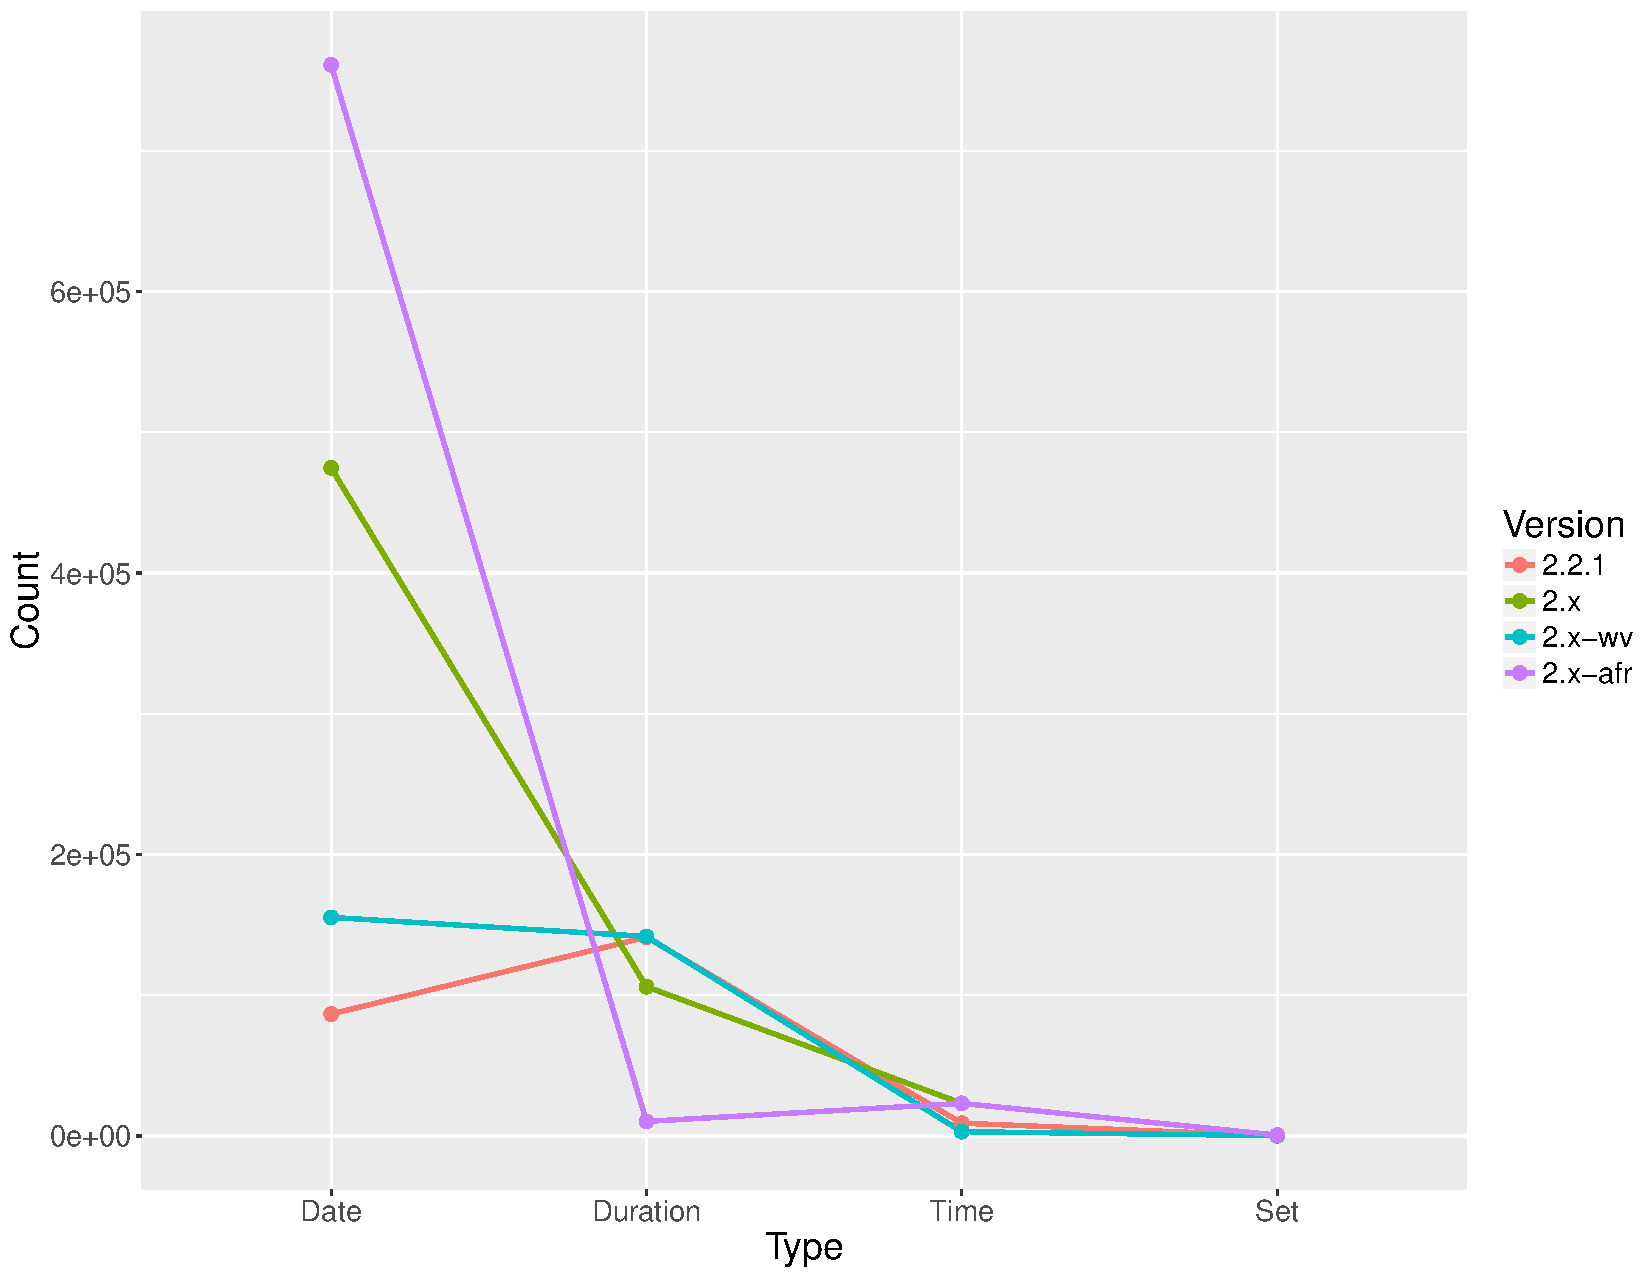
\includegraphics[width=14cm]{Plots/polish-tempex-type-landscape}
	\caption{Distribution of temporal expressions extracted per type using HeidelTime's different versions of automatically developed resources - for Polish Wikipedia dump.}
	\label{figure:5a}
\end{figure}

The Figure \ref{figure:5a}, shows that the general pattern of lineplots for version 2.x and 2.x-afr is similar to the distribution of temporal expressions in WikiWars corpus by Mazur and Dale in \cite{mazur2010wikiwars}, i.e., a major portion of temporal expressions are of DATE type, and rest are of DURATION, TIME and SET types.

In the following table, we present some more findings on tagging of Polish, Czech and Finnish Wikipedia dumps.

\begin{table}[H]
	\centering
	%	\rowcolors{1}{}{cream}
	\begin{threeparttable}
		\begin{tabularx}{300pt}{|| >{\raggedright\arraybackslash}p{.5in} >{\raggedright\arraybackslash}p{.6in} | >{\raggedleft\arraybackslash}X | >{\raggedleft\arraybackslash}X | >{\raggedleft\arraybackslash}X   ||} 
			\hline
			\multicolumn{2}{||c}{\multirow{2}{*}{}} & \multicolumn{1}{c}{\#3} & \multicolumn{1}{c}{\#4} & \multicolumn{1}{c||}{\#5} \\ [0.5ex] 
			%			\hline
			\textbf{lang.} & \textbf{version} & \textbf{\% of docs tagged} & \textbf{avg. no. tempexs per doc} & \textbf{count YYYY-MM-DD}\\ 
			\hline\hline
			
			\multirow{4}{\linewidth}{Polish} & 2.2.1 & 6.29 & 3.03 & \num[group-separator={,}]{10644} \\ 
			\cline{2-5} & 2.x & 11.27 & 4.32 & \num[group-separator={,}]{333613} \\ 
			\cline{2-5} & 2.x-wv  & 7.99 & 3.03 & \num[group-separator={,}]{0} \\  
			\cline{2-5} & 2.x-afr  & 12.86 & 4.98 & \num[group-separator={,}]{338969} \\  
			\hline\hline
			
			\multirow{4}{\linewidth}{Czech} & 2.2.1 & 7.09 & 2.48 & \num[group-separator={,}]{27815} \\ 
			\cline{2-5} & 2.x & 13.62 & 4.46 & \num[group-separator={,}]{163938} \\  
			\cline{2-5} & 2.x-afr & 16.69 & 6.12 & \num[group-separator={,}]{165927} \\ 
			\hline\hline
			
			\multirow{4}{\linewidth}{Finnish} & 2.2.1 & 7.62 & 1.88 & \num[group-separator={,}]{16817} \\ 
			\cline{2-5} & 2.x & 52.98 & 3.39 & \num[group-separator={,}]{420702} \\ 
			\cline{2-5} & 2.x-wv  & 48.27 & 2.79 & \num[group-separator={,}]{58} \\  
			\cline{2-5} & 2.x-afr  & 74.97 & 5.02 & \num[group-separator={,}]{429699} \\ 
			\hline\hline
			
		\end{tabularx}
		%		\begin{tablenotes}
		%			\item[1] for unsegmented languages, the rules do not use space as separator between rePatterns
		%		\end{tablenotes}
	\end{threeparttable}
	\caption{Results of Wikipedia dumps for some languages of Europe (2/2).}
	\label{table:5-results-wikis345-europe}
\end{table}

The Table \ref{table:5-results-wikis345-europe}, shows that using 2.x and 2.x-afr version resources resulted in tagging higher percentage of total Wikipedia documents of respective languages, getting higher average number of temporal expressions tagged per document, normalizing higher number of temporal expressions to the YYYY-MM-DD format. 

In total, the Wikipedia evaluations were ran for 177 languages. These many languages had their respective Wikipedia dumps, dated 2017-10-20, available. Some further Wikipedia dumps evaluation tables for additional languages, chosen arbitrarily, are given in Appendix \ref{wiki-appendix}.

\section{Summary}
In this chapter, we described our experiments and evaluation results. We started the chapter with the description of our evaluation approach, that summarized the different versions of HeidelTime resources that we would evaluate and compare in following sections. In second section, we discussed the evaluation measures such as precison, recall and F\textsubscript{1} score; then, we discussed the difference between strict and relaxed matching while computing the described evaluation measures; finally, we summarized the evaluations on temporally annotated corpora. We noted that the new version of resources, especially the version 2.x-afr performed better in majority of the corpora thus effectively improving the baseline tagging performance over version 2.2.1 resources. In third section, we summarized the experiment results on Wikipedia dumps for some languages. We observed that the version 2.x resources performed good for morphologically rich languages. And version 2.x-afr resources extracted even more overall temporal expressions as compared to version 2.x resources. 
